This chapter shows the results of the simulations done with the framework shown in ch. \ref{ch:methodology} as well as discussing the results.
The chapter is mainly divided into two sections, the first explaining the configuration of the simulation as well as results depicted by graph-data.
The second section focuses on discussing the results in terms of the reason they have certain values and graphs, as well as a comparison between the different simulations and discovery of correlations and behavioural similarities.

\section{Experimental Results}
As stated in the chapter introduction, this section covers the results of the simulations. 
Even though the simulator supports a wide variety of different configurations, three main simulation groups chosen for this particular study.
The first group considers different connection port configurations for the robots.
The second simulation group varies the environment that the robots spend their life time in.
The third and final simulation group aims to observe the affect of local communication between the robots in a self-assembly structure(the implementation is shown in sec. \ref{sec:local_comm}).
The two first simulation groups targets to contribute to the three main self-assembly mechanisms discussed in ch. \ref{ch:background}(Self-assembly Architectures, Hardware Mechanisms and Assembly Protocols).
The local communication simulation group aims to study the affect giving the robots the ability to perform simple communication between the robots in a group.

\subsection{Port Configuration}
The first group of simulations that were done was varying the number of connection ports of the robots and their configuration.
These simulations where done such that one could record and discuss the impact of connections between the robots.
In more detail, this group of experiments where conducted such that one could record:

\begin{itemize}
	\item How the number of ports affected the general performance of the system based on the number of ports.
	\item If there is any noticeable difference in the self-assembly architecture.
	\item In what way the port configuration promotes self-assembly, both in therms of the sizes of the different robot groups, and the number of groups.
	\item How the port configuration affect the fitness of the sexperiment, in terms of convergence and final result.
\end{itemize}

The goal of running these simulations is to make correlations between its results to show how configuring the hardware mechanism can affect a self-assembly system.
 
For this group of simulations, the most relevant statistics will be the difference between group actions versus single robot actions.
The following pages show the recorded data for simulations using, 2 connection ports, 3 connection ports and 4 connection ports.


\begin{figure}[H]
	\centering
	\begin{subfigure}[b]{0.31\textwidth}
		\centering
		\fbox{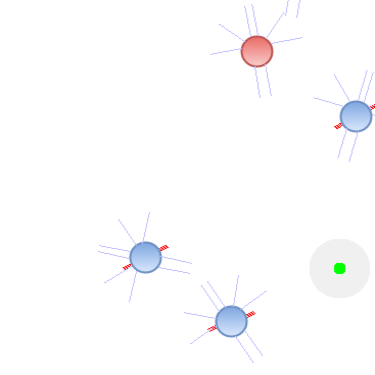
\includegraphics[height=\linewidth]{chapters/res/2-conn.png}}
		\caption{2-ports}
	\end{subfigure}
	\begin{subfigure}[b]{0.31\textwidth}
		\centering
		\fbox{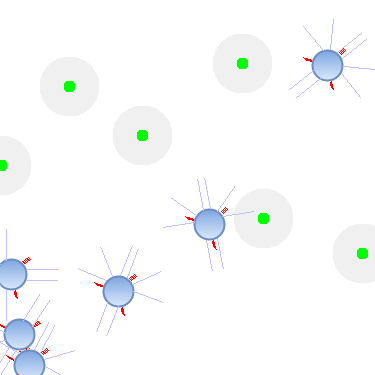
\includegraphics[height=\linewidth]{chapters/res/3-conn.png}}
		\caption{3-ports}
	\end{subfigure}
	\begin{subfigure}[b]{0.31\textwidth}
		\centering
		\fbox{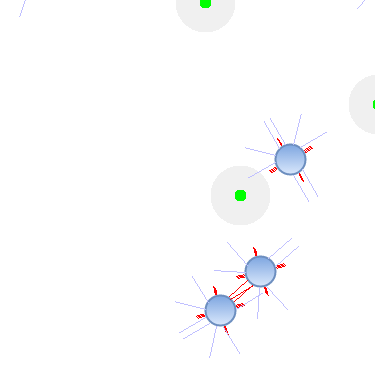
\includegraphics[height=\linewidth]{chapters/res/4-conn.png}}
		\caption{4-ports}
	\end{subfigure}
	\caption{The three different port configurations used in simulation}
	\label{fig:collective-behaviour}
\end{figure}


Common configuration parameters of importance for the simulations are listed in table \ref{port-eniornment-config}.

\begin{table}[H]
	\centering
	\begin{tabular}{|c|c|}
		\hline Parameter & Value \\ 
		\hline Number of Robots & 20 \\ 
		\hline Iterations per Generation & 10000 \\
		\hline Scenarios & 3 \\ 
		\hline Generations & 150 \\ 
		\hline 
		
	\end{tabular}
	\caption{The simulation parameters for the environments.}
	\label{port-eniornment-config}
\end{table}



\newpage

\pagestyle{plain}

\vspace*{\fill}
\begin{center}
	\subsubsection{Fitness}
	\vspace*{-0.6cm}
\end{center}

\insertresultgraphs{chapters/generated-graphs/2-ports/fitness-out-2-ports.tex}{chapters/generated-graphs/3-ports/fitness-out-3-ports.tex}{chapters/generated-graphs/4-ports/fitness-out-4-ports.tex}{Figure shows "fitness" results from connection port simulations}
\vspace*{\fill}
\newpage
\vspace*{\fill}
\begin{center}
	\subsubsection{Group Distribution}
	\vspace*{-0.6cm}
\end{center}

\insertresultgraphs{chapters/generated-graphs/2-ports/group_distribution-out-2-ports.tex}{chapters/generated-graphs/3-ports/group_distribution-out-3-ports.tex}{chapters/generated-graphs/4-ports/group_distribution-out-4-ports.tex}{Figure shows "group distribution" results from connection port simulations}
\vspace*{\fill}
\newpage
\vspace*{\fill}
\begin{center}
	\subsubsection{Number of Groups}
	\vspace*{-0.6cm}
\end{center}

\insertresultgraphs{chapters/generated-graphs/2-ports/number_of_groups-out-2-ports.tex}{chapters/generated-graphs/3-ports/number_of_groups-out-3-ports.tex}{chapters/generated-graphs/4-ports/number_of_groups-out-4-ports.tex}{Figure shows "number of groups" results from connection port simulations}
\vspace*{\fill}
\newpage
\vspace*{\fill}
\begin{center}
	\subsubsection{Robots Eaten}
	\vspace*{-0.6cm}
\end{center}

\insertresultgraphs{chapters/generated-graphs/2-ports/robots_eaten-out-2-ports.tex}{chapters/generated-graphs/3-ports/robots_eaten-out-3-ports.tex}{chapters/generated-graphs/4-ports/robots_eaten-out-4-ports.tex}{Figure shows "robots eaten" results from connection port simulations}
\vspace*{\fill}
\newpage
\vspace*{\fill}
\begin{center}
	\subsubsection{Robots Starved}
	\vspace*{-0.6cm}
\end{center}

\insertresultgraphs{chapters/generated-graphs/2-ports/robots_starved-out-2-ports.tex}{chapters/generated-graphs/3-ports/robots_starved-out-3-ports.tex}{chapters/generated-graphs/4-ports/robots_starved-out-4-ports.tex}{Figure shows "robots starved" results from connection port simulations}
\vspace*{\fill}
\newpage
\vspace*{\fill}
\begin{center}
	\subsubsection{Energy Consumed by Group}
	\vspace*{-0.6cm}
\end{center}

\insertresultgraphs{chapters/generated-graphs/2-ports/energy_consumed_by_group-out-2-ports.tex}{chapters/generated-graphs/3-ports/energy_consumed_by_group-out-3-ports.tex}{chapters/generated-graphs/4-ports/energy_consumed_by_group-out-4-ports.tex}{Figure shows "energy consumed by group" results from connection port simulations}
\vspace*{\fill}
\newpage
\vspace*{\fill}

\begin{center}
	\subsubsection{Energy Consumed by Robot}
	\vspace*{-0.6cm}
\end{center}

\insertresultgraphs{chapters/generated-graphs/2-ports/energy_consumed_by_robot-out-2-ports.tex}{chapters/generated-graphs/3-ports/energy_consumed_by_robot-out-3-ports.tex}{chapters/generated-graphs/4-ports/energy_consumed_by_robot-out-4-ports.tex}{Figure shows "energy consumed by robot" results from connection port simulations}
\vspace*{\fill}
\newpage
\vspace*{\fill}
\begin{center}
	\subsubsection{Predators Eaten}
	\vspace*{-0.6cm}
\end{center}

\insertresultgraphs{chapters/generated-graphs/2-ports/predators_eaten-out-2-ports.tex}{chapters/generated-graphs/3-ports/predators_eaten-out-3-ports.tex}{chapters/generated-graphs/4-ports/predators_eaten-out-4-ports.tex}{Figure shows "predators eaten" results from connection port simulations}
\vspace*{\fill}


\newpage

\pagestyle{main}

\subsection{Environment Difficulty}
The motivation for this experiment is to observe how changing the difficulty of the environment affects the evolved behaviour.
For the experiment two environment difficulties were constructed, one easier and one more difficult.
These environment difficulties were then used in the simulations so that the impact of the evolutionary pressure could be recorded and discussed.
More specifically the experiments were constructed to investigate how differing environment difficulties affect the following properties of the evolved behaviour.

\begin{itemize}
	\item The amount of robot groups formed through self-assembly, and the number of robots in each group.
	\item How the energy gathering behaviour is affected. Whether the robots prefer gathering energy individually, or as robot groups. 
	\item How the environment difficulty affects the fitness of the experiment, in terms of convergence and final result.
\end{itemize}


The environment difficulty is modified by varying the following simulation parameters.
The initial energy level the robots, the maximum amount of energy each robot can be charged with, the amount of food in the environment, and the number of predators present in the simulation.
Table \ref{tab:environment-difficulty} presents the simulation parameters that are varied for the environments.

\begin{table}[H]
	\centering

	\begin{tabular}{|c|c|c|c|c|}
		\hline  & \small{Predators} & \small{Initial energy} & \small{Food items} & \small{Maximum energy} \\ 
		\hline \small{Easy environment} & 4 & 8000 & 25 & 10000 \\ 
		\hline \small{Hard environment} & 7 & 6000 & 20 &8000 \\ 
		\hline 
		
	\end{tabular} 
	\caption{The simulation parameters for the environments.}
	\label{tab:environment-difficulty}
\end{table}

The results were obtained by running 20 simulation trials for each difficulty, where each of the trails run for 150 generations.

\newpage
\pagestyle{plain}

\vspace*{\fill}

	\begin{center}
		\subsubsection{Fitness}
		\vspace*{-0.6cm}
	\end{center}

	\insertresultgraphstwo{chapters/generated-graphs/easy/fitness-easy-out.tex}{chapters/generated-graphs/hard/fitness-hard-out.tex}{Figure shows "fitness" results from connection port simulations}{fitness}

%These graphs show the results for achieved fitness for the environment difficulty simulations.
%The easy environment result is similar to 
\vspace*{\fill}

\newpage
\vspace*{\fill}
\begin{center}
	\subsubsection{Group Distribution}
	\vspace*{-0.6cm}
\end{center}

\insertresultgraphstwo{chapters/generated-graphs/easy/group_distribution-easy-out.tex}{chapters/generated-graphs/hard/group_distribution-hard-out.tex}{Figure shows "group distribution" results from connection port simulations}{group-distribution}
\vspace*{\fill}
\newpage
\vspace*{\fill}
\begin{center}
	\subsubsection{Number of Groups}
	\vspace*{-0.6cm}
\end{center}

\insertresultgraphstwo{chapters/generated-graphs/easy/number_of_groups-easy-out.tex}{chapters/generated-graphs/hard/number_of_groups-hard-out.tex}{Figure shows "number of groups" results from connection port simulations}{number-of-groups}
\vspace*{\fill}
\newpage
\vspace*{\fill}
\begin{center}
	\subsubsection{Robots Eaten}
	\vspace*{-0.6cm}
\end{center}

\insertresultgraphstwo{chapters/generated-graphs/easy/robots_eaten-easy-out.tex}{chapters/generated-graphs/hard/robots_eaten-hard-out.tex}{Figure shows "robots eaten" results from connection port simulations}{robots-eaten}
\vspace*{\fill}
\newpage
\vspace*{\fill}
\begin{center}
	\subsubsection{Robots Starved}
	\vspace*{-0.6cm}
\end{center}

\insertresultgraphstwo{chapters/generated-graphs/easy/robots_starved-easy-out.tex}{chapters/generated-graphs/hard/robots_starved-hard-out.tex}{Figure shows "robots starved" results from connection port simulations}{robots-starved}
\vspace*{\fill}
\newpage
\vspace*{\fill}
\begin{center}
	\subsubsection{Energy Consumed by Group}
	\vspace*{-0.6cm}
\end{center}

\insertresultgraphstwo{chapters/generated-graphs/easy/energy_consumed_by_group-easy-out.tex}{chapters/generated-graphs/hard/energy_consumed_by_group-hard-out.tex}{Figure shows "energy consumed by group" results from connection port simulations}{energy-consumed-by-group}
\vspace*{\fill}
\newpage
\vspace*{\fill}

\begin{center}
	\subsubsection{Energy Consumed by Robot}
	\vspace*{-0.6cm}
\end{center}

\insertresultgraphstwo{chapters/generated-graphs/easy/energy_consumed_by_robot-easy-out.tex}{chapters/generated-graphs/hard/energy_consumed_by_robot-hard-out.tex}{Figure shows "energy consumed by robot" results from connection port simulations}{energy-consumed-by-robot}
\vspace*{\fill}
\newpage
\vspace*{\fill}
\begin{center}
	\subsubsection{Predators Eaten}
	\vspace*{-0.6cm}
\end{center}

\insertresultgraphstwo{chapters/generated-graphs/easy/predators_eaten-easy-out.tex}{chapters/generated-graphs/hard/predators_eaten-hard-out.tex}{Figure shows "predators eaten" results from connection port simulations}{predators-eaten}
\vspace*{\fill}


\newpage
\pagestyle{main}

\subsection{Local Communication}
\label{sec:local_communication}
The goal of this experiment is to investigate the impact local communication has on the behaviour of the robots.
The experiment is performed by selecting the fittest genomes found for the environments, and observing the change, if any, in robot behaviour when the local communication is disabled.


The behaviour observed in the easy and difficult environment is very similar.
Therefore the description of the observed behaviour is combined into one section.
The robots rarely disconnect once they are in a robot group.
Their behaviour can be split into two phases, the individual behaviour, and the group behaviour.

\subsubsection{Individual behaviour}
\label{sec:invdividual_behaviour}
The individual robots have two observed movement "modes".
Which one is used depends on if a wall is within sensor range.
If no walls are detected the robots will drive in wide circles.
In this mode the robots collect energy, and will attempt connections with other robots they crash into.
However, they make no attempt to avoid predators in their path.
This behaviour is usually observed at the beginning of the simulation since most of the robots are initialized away from the walls.


The circles the robots drive in are wide enough to make them crash into the walls of the environment.
Once a wall is detected by the sensors, the behaviour changes.
Instead of driving in circles the robot will now drive along the wall of the environment.
Figure \ref{fig:individual-wall-drive} shows how a robot follows the wall while keeping it in sensors range.

\begin{figure}[H]	
	\centering
	\fbox{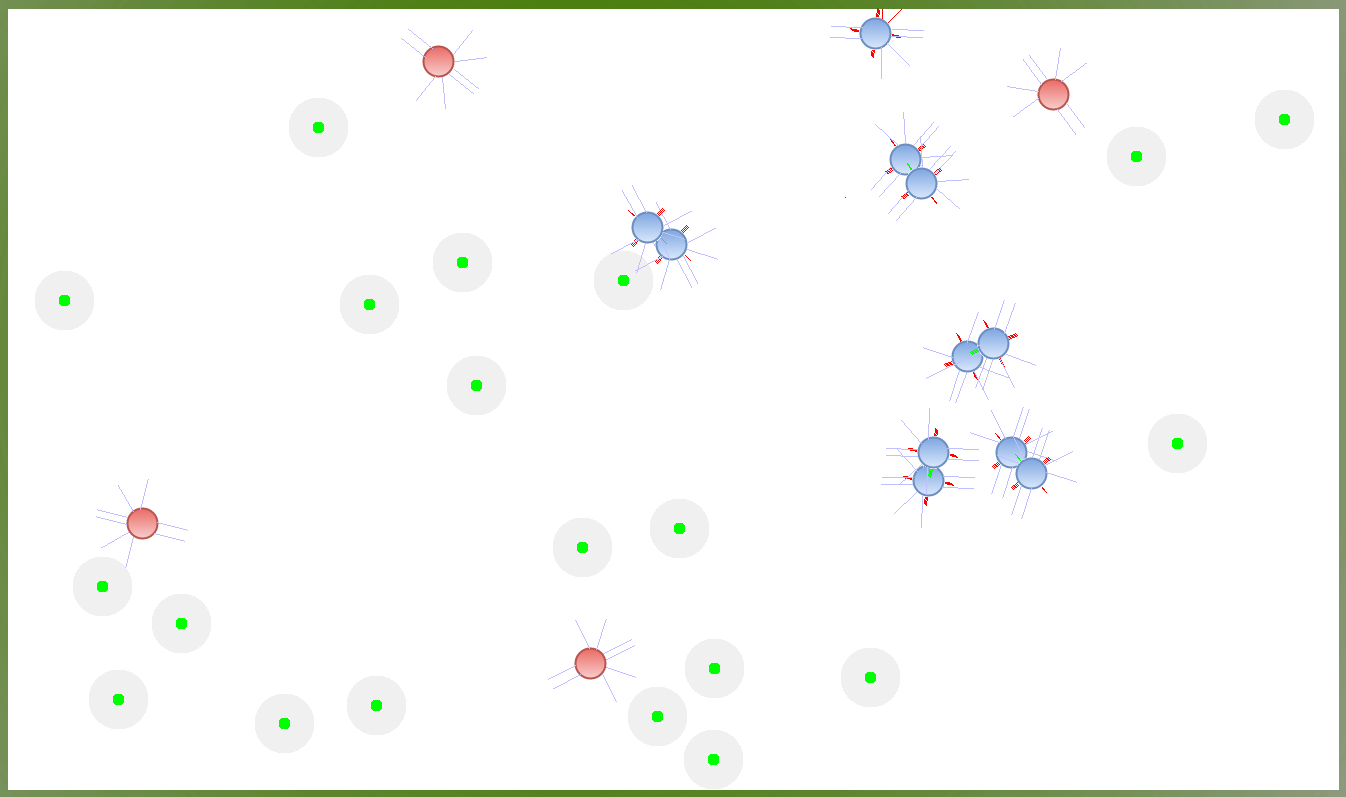
\includegraphics[width=0.65\textwidth]{chapters/res/wall-hug.png}}
	\caption{A robot using its sensors to follow a wall.}
	\label{fig:individual-wall-drive}
\end{figure}


The robot will keep on driving along the wall until it meets another robot, and is able to form a group, or if the sensors detect a robot group passing by.
If a robot group comes within sensor range wile the robot is driving along the wall, the robot will abandon the wall and attempt to follow the group instead.

\subsubsection{Group behaviour}


\begin{figure}[H]
	
	\centering
	\fbox{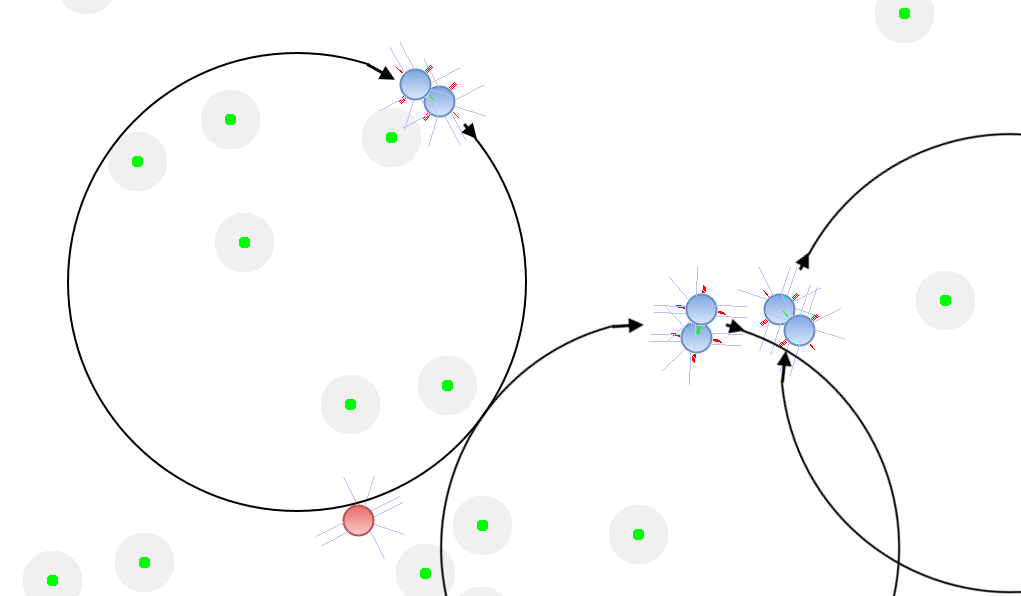
\includegraphics[width=0.65\textwidth]{chapters/res/group_circles.png}}
	\caption{Robot groups driving in circles.}
	\label{fig:group-circles}
\end{figure}

The behaviour of the robot groups is similar to the first mode of the individual robots.
Robot groups also drive in wide circles, displayed in figure \ref{fig:group-circles}, but if the group crashes into a wall it will simply turn around and continue.
The robot groups consume predators in their path, but they make no attempt to follow detected predators.
The robot groups will continue to drive in circles, consuming energy, predators, and making connections, until the end of the simulation, or until the members of the groups starve.

\subsubsection{Local communication}
\label{sec:disable-local-communication}
Disabling the local communication module has a significant effect on the behaviour.
With the communication disabled the robots will no longer switch to the group behaviour once they are connected.
Instead the groups will continue to perform the individual robot behaviour regardless of the number of connected robots.

\section{Discussion}

\subsection{Environmental difficulty analysis}
\subsubsection{Environmental threats}
The robots have two threats in the environments presented, starvation and getting killed by predators.
The robots in the easy environment receive more energy from food, and there is more food available.
From figure \ref{fig:robots-starved-easy} and figure \ref{fig:robots-starved-hard} one can see that this reduces the amount of robots dying from starvation in the easy environment, but the improvement is minuscule.

Increasing the number of predators in the environment seems to have a higher impact on the difficulty presented by an environment.
Figure \ref{fig:robots-eaten-easy} and figure \ref{fig:robots-eaten-hard} shows that increasing the amount of predators present in the environment has a greater impact on the difficulty of the environment than limiting the energy available.
The reason for why increasing the amount of predators has a much higher impact on difficulty is not completely clear from the results.
However, the observed behaviour described in section \ref{sec:invdividual_behaviour} can help explain the results.
The sensors are used by the robot to detect walls and other robots, but not predators or food.
This means that the robot may miss some food, but there is enough food in the environment so the robot will eventually find more food.
On the other hand, failing at predator avoidance has much more severe consequences as the predator will kill the robot.

\subsubsection{Promotion of self-assembly}
One of the motivations for this experiment was to see how modifying the evolutionary pressure affects the promotion of self-assembly.
The figures \ref{fig:number-of-groups-easy} and \ref{fig:number-of-groups-hard} shows that the robots form more groups in the easy environment.
At first glance this seems to indicate that the easy environment is more successful at promoting self-assembly.
This difference in number of groups may be explained by examining the lifetime of the robots.
As explained in section \ref{sec:evaluation}, the fitness of a genome is determined by the average lifetime of a robot.
The fitness achieved in the easy environment, figure \ref{fig:fitness-easy}, is higher than than the fitness achieved in the hard environment, figure \ref{fig:fitness-hard}.
This means that the robots in the easy environment live longer, and as a consequence have more time to form groups.

However, figure \ref{fig:group-distribution-easy} and figure \ref{fig:group-distribution-hard} shows that the size of the robot groups formed are not affected by modifying the difficulty of the environment.
In both environments the distribution of group sizes are heavily weighted towards groups of two.
The reason for this may be that the environments gives a high reward for being in a group.
That is protection from predators, but there is no additional reward for forming larger groups.

\subsubsection{Energy collection strategy}
One can see from the figures \ref{fig:energy-consumed-by-robot-easy}, \ref{fig:energy-consumed-by-group-easy} and \ref{fig:energy-consumed-by-robot-hard}, \ref{fig:energy-consumed-by-group-hard} that the robots in the easy environment collect far more energy than the robots in the difficult environment as individual robots and in robot groups.
This result can likely also be attributed to the fact that the robots in the easy environment live longer, and that there is more energy available, instead of a more optimal energy gathering strategy.
The reasoning for this is as follows.
The ratio of energy consumed by individual robots and energy consumed by groups in the best case at the final generation for the environments are both at 73\% of energy being collected by the groups.
This means that although the robots in the easy environment collect more energy, the strategies evolved in the different environments are similar.
This also coincides with with that the observed behaviour described in section \ref{sec:local_communication} is very similar for the different environments.

\subsection{Local communication analysis}
As described in section \ref{sec:disable-local-communication}, the evolved behaviour makes use of the communication module.
When the communication module was disabled, the robots did not change their behaviour when they formed groups.
Therefore it is reasonable to assume that local communication is at least involved in modifying the robot behaviour once connected to a group.
Exactly how the evolved neural network interprets the messages received is difficult to infer, but one can have a look at the messages sent to get an overview.

\begin{figure}[H]
	\centering
	[0.992 0.999 0.423 0.002]
	\label{fig:message_default}
	\caption{The message passed between the robots.}	
\end{figure}

Without any other inputs all robots send the message displayed in \ref{fig:message_default} by default.
Receiving other inputs, such as sensors, changes the by a negligible amount.
The surprising thing about the message is that the components in the message have wildly different values.
It turns out that the values in the messages has an interesting interaction with the port connection status that is also given to the neural network.
The port connection status contains the connection status of each port the robot has.

\begin{table}[H]	
		
	\begin{tabular}{c c}
			\hline
			Message:[0.992 0.999 0.423 0.002] & Message: [1 1 1 1] \\
				\hline
		\begin{tabular}[t]{|c|c|}
		
			\hline \small{Desired rotation} \tiny{deg/step} & \small{Port status} \\ 
			\hline 0.9482 & [1 1 0 0] \\ 
			\hline 0.999 & [1 0 1 0] \\ 
			\hline 0.517 & [1 0 0 1] \\ 
			\hline 0.997 & [0 1 1 0] \\ 
			\hline 0.705 & [0 1 0 1] \\ 
			\hline 0.997 & [0 0 1 1] \\ 
			\hline 
		\end{tabular} 
			&
		\begin{tabular}[t]{|c|c|}
		
			\hline \small{Desired rotation} \tiny{deg/step} & \small{Port status} \\ 
			\hline 0.719 & [1 1 0 0] \\ 
			\hline 0.976 & [1 0 1 0] \\ 
			\hline 0.658 & [1 0 0 1] \\ 
			\hline 0.866 & [0 1 1 0] \\ 
			\hline 0.674 & [0 1 0 1] \\ 
			\hline 0.822 & [0 0 1 1] \\ 
			\hline 	
		\end{tabular} 	
	\end{tabular}
		\caption{The resulting desired rotations for different port combinations with the evolved message and a test message for comparison.}
		\label{tab:port-desired-rotation}
\end{table}

Table \ref{tab:port-desired-rotation} shows how the desired rotation for the robots varies with the local topology of the connected robots.
The table shows this variation with the evolved message, and a dummy message for comparison.
One can se that the resulting desired rotation for the robots has different values for the two messages.
The desired rotation for the robots determine the radius of the circles the robot groups move in.
This shows that the local communication module is used for two purposes.
The first purpose is to act as a switch to change from the individual robot behaviour, to the group behaviour.
Additionally, the message passed around decides the radius of the circles the robots move in for different connection topologies.


\subsection{Port configuration Analysis}
In terms of the results fetched from the port configuration simulations the first obvious remarks stem from the simulation running a three port configuration.
The results in this simulation is much weaker in terms of performance and in terms of promoting self-assembly than the simulations running 2 and 4 connection ports.
The reason for this can not be deduced completely from the empirical results, but as the only difference in these simulations are the number of ports and the alignment it is clear that the connection port configuration can greatly impact the performance of the simulation.
It can also be deduced that it is not the number of connection ports that has the primary impact of the solution, but rather the placement.
The reason one can make this claim is because the configuration using 2 connection ports and 4 connection ports perform quite similar in terms of performance.
If the number of connection ports had a great impact on the results, one would expect the simulation using 2 connection ports or 4 connection ports to yield even poorer results than the 3 connection port simulation.
This narrows the port configuration problem down to the alignment of the connection ports.

\begin{figure}[H]
	\centering
	\begin{subfigure}[b]{0.31\textwidth}
		\centering
		\fbox{\includegraphics[height=\linewidth]{chapters/res/2-ports-robot.png}}
		\caption{2-ports}
	\end{subfigure}
	\begin{subfigure}[b]{0.31\textwidth}
		\centering
		\fbox{\includegraphics[height=\linewidth]{chapters/res/3-ports-robot.png}}
		\caption{3-ports}
	\end{subfigure}
	\begin{subfigure}[b]{0.31\textwidth}
		\centering
		\fbox{\includegraphics[height=\linewidth]{chapters/res/4-ports-robot.png}}
		\caption{4-ports}
	\end{subfigure}
	\caption{The three different port configurations used in simulation}
	\label{fig:robot-port-configuration}
\end{figure}

Figure \ref{fig:robot-port-configuration} shows a closer view of the alignment that the robots initially have when spawned into the environment.
As explained in \ref{sec:modifications}, the robots can rotate their connection ports as a group.
A standard strategy which is usually evolved is to either constantly rotate the connection ports in hopes of lining up the ports to another robot, or, the robots start rotating their ports when the sensors see another robot in an effort to self-assemble.
There are two main problems that the 3 connection port robots have compared to the other port configurations.
First, the initial port location does not align to any other robot.


\begin{figure}[H]
	\begin{subfigure}[t]{0.49\textwidth}
		\centering
		\fbox{\includegraphics[height=0.9\linewidth]{chapters/res/3-ports-alignment.png}}
		\caption{Initial alignment}
		\label{3-port-guided-allignment}
	\end{subfigure}
	\begin{subfigure}[t]{0.49\textwidth}
		\centering
		\fbox{\includegraphics[height=0.9\linewidth]{chapters/res/3-ports-alignment-offset.png}}
		\caption{After $50^{\circ}$ port rotation.}
		\label{3-port-guided-allignment-offset}
	\end{subfigure}
	\caption{This figure shows how the 3 connection port robots align}
\end{figure}


As seen in figure \ref{3-port-guided-allignment}, there is not a trivial alignment for the robots to connect.
One might initially presume that this is not a problem as the robots have a mechanism for rotating their ports to solve this exact issue.
However, as all the robots are running the same genome, as per off-line evolution and hence the same behaviour, it becomes increasingly difficult for the robots to solve this problem.
As explained earlier, the robots in this simulation tend to evolve a strategy which involves constantly spinning the connection ports in one direction.
But, as seen in figure \ref{3-port-guided-allignment-offset}, in the case where all robots at some time step have rotated their connection ports $50^{\circ}$, the same issue of port alignment would still hold.

\begin{figure}[H]
	\begin{subfigure}[t]{0.49\textwidth}
		\centering
		\fbox{\includegraphics[height=0.9\linewidth]{chapters/res/2-ports-alignment.png}}
		\caption{2 connection ports alignment}
		\label{2-port-guided-allignment}
	\end{subfigure}
	\begin{subfigure}[t]{0.49\textwidth}
		\centering
		\fbox{\includegraphics[height=0.9\linewidth]{chapters/res/4-ports-alignment.png}}
		\caption{4 connection ports alignment}
		\label{4-port-guided-allignment}
	\end{subfigure}
	\caption{This figure shows how the 2 and 4 connection ports robots align from initial configuration}
	\label{2-4-port-guided-allignment}
\end{figure}

Consider figure \ref{2-4-port-guided-allignment}.
In this example there are two and four port configurations.
It can be observed that with initial rotation of the ports, there exists possibilities for the robots to self-assemble without having the robots behave differently in terms of rotating their connection ports.
This differentiation seems to be the main reason that the 3 connection port configuration is being outperformed.

The second problem robots with 3 connection ports, in this alignment, is the possible group formations the robots can form.
Chapter \ref{ch:background} covers the chain and lattice architectures that the robots can form when self-assembling. %needs ref/explain
The simulator is developed to support the lattice architecture because if its simplistic method of coordinated movement.

\begin{figure}[H]
	\begin{subfigure}[t]{0.49\textwidth}
		\centering
		\fbox{\includegraphics[height=0.9\linewidth]{chapters/res/2-4-port-architectures.png}}
		\caption{Robot groups with 2 and 4 connection ports}
		\label{2-4-port-architecture}
	\end{subfigure}
	\begin{subfigure}[t]{0.49\textwidth}
		\centering
		\fbox{\includegraphics[height=0.9\linewidth]{chapters/res/3-ports-architecture.png}}
		\caption{Robot groups with 3 connection ports}
		\label{3-port-architecture}
	\end{subfigure}
	\caption{This figure contains self-assembled robot groups with different assembly combinations}
	\label{port-architectures}
\end{figure}

It can be seen from figure \ref{port-architectures} that the different connection port configurations creates different types of groups. 
With 2 and 4 connection ports (figure \ref{2-4-port-architecture}), the robot groups either take the form of a line or some square grid formation.
Possible formations of the 3 connection ports robot groups(figure \ref{3-port-architecture}) brakes the pattern of a square grid configuration which makes it harder for other robots trying to connect to the group.
The main reason for this connection problem is the relative position a connecting robot needs, is harder to attain because of the larger distance between the connection ports.

There are not large discrepancies between the results from the port configuration simulation containing 2 and 4 connection ports.
The only result which differs significantly is "predators eaten"(figure \ref{fig:predators-eaten-2-ports} and \ref{fig:predators-eaten-4-ports}).
The reason for this can be deduced from figure \ref{fig:group-distribution-2-ports} and \ref{fig:group-distribution-4-ports} which shows that robots with 4 connection ports tend to form larger groups.
It can however be viewed from figure \ref{fig:number-of-groups-2-ports} and \ref{fig:number-of-groups-4-ports} that 2 and 4 connection ports have roughly the same number of groups.
The occurrence of a greater amount of larger groups naturally agrees with eaten more predators as groups need to be of at least size three to consume a predator.
The reason for 4 connection ports robots to attain larger groups is simply that more connection ports yields more points of entry for other robots trying to connect, which increases the probability of succeeding self-assembly to the group.

From these results, it can be deduced that larger groups do not give rise to better fitness in this experiment, but rather the number of groups (a group is of minimum size 2) correlates with the fitness.
The reason for this is that the robots in the port configuration simulations are not in a great need of energy.
The are able to naturally attain what they need in the environment and hence do not have to rely on a strategy involving predator consumption.

























